\chapter{Introdução}
\label{cap:introdução}

%\pretextualchapter{Hiram}

Este capítulo descreve um breve resumo dos principais pontos do contexto global onde este trabalho está inserido, começando por identificar a criação dos sistemas evolutivos na União Europeia (UE) e os sistemas ciber-físicos nos Estados Unidos da América (EUA). Após o que, relaciona essas estratégias globais com o as estratégias brasileiras e reconhece-se a quase inexistência de dispositivos e protótipos que permitam à academia realizar os estudos e as pesquisas necessárias para a indústria brasileira se adaptar às recomendações da Indústria 4.0 (\iQuatroZero). Por fim identifica o tema, descreve o problema a ser tratado por esse trabalho, as questões de pesquisa, os objetivos geral e específicos, descreve a proposta de trabalho, as motivações, a metodologia utilizada, cita as principais contribuições e resume os demais capítulos que fazem parte desta pesquisa. 


%===================================================================

\section{Contextualização Global}
 
Até o final da década de 80 os sistemas flexíveis conseguiam resolver o principal problema das empresas industriais até então: a produção em lotes médios e pequenos. Contudo, a partir de 1989, intensificou-se a troca de bens entre diferentes continentes e as exigências dos clientes levou ao aumento do nível de customização. Além disso, tecnologias como a Internet aproximaram mercados e consumidores de locais distantes. A troca rápida de informações e os ativos intangíveis transformaram a economia mundial numa rede global de conhecimento~\cite{Abele}.

Para fazer frente a esses novos desafios, naturalmente houve o desenvolvimento de novas formas de se olhar a manufatura. Essas novas forma são conhecidas como os paradigmas da manufatura cujos surgimentos estão ilustrados  na Figura~\ref{fig:paradigmas_producao}. Nela estão enfatizados o paradigma \textit{FMS} e o surgimento dos paradigmas emergentes \textit{(HMS, BMS e RMS)}. Esses paradigmas inovaram ao desconsiderar os equipamento da manufatura como detentores da inteligência para a montagem, isto é, o conhecimento do processo produtivo. Nesses paradigmas e, em especial no paradigma \textit{EPS}, o foco da inteligência foi direcionado para o produto, que detém o conhecimento da montagem de si mesmo e não mais as ferramentas de montagem. 

Também os sistemas evolutivos passam a ter, atualmente, maior relevância no tratamento do problema da customização e estão sendo testados objetivando as indústrias inteligentes e as exigências da Indústria 4.0. Mais recentemente surgiu um novo paradigma denominado de \textit{SAS (Symbiotic Assembly System)}~\cite{FERREIRA2014} que procura integrar os sistemas de automação rígido, flexível e programável às capacidades do ser humano. % que neste paradigma faz parte ativa da modelagem.

%================================================================
\begin{figure*}
	\centering
	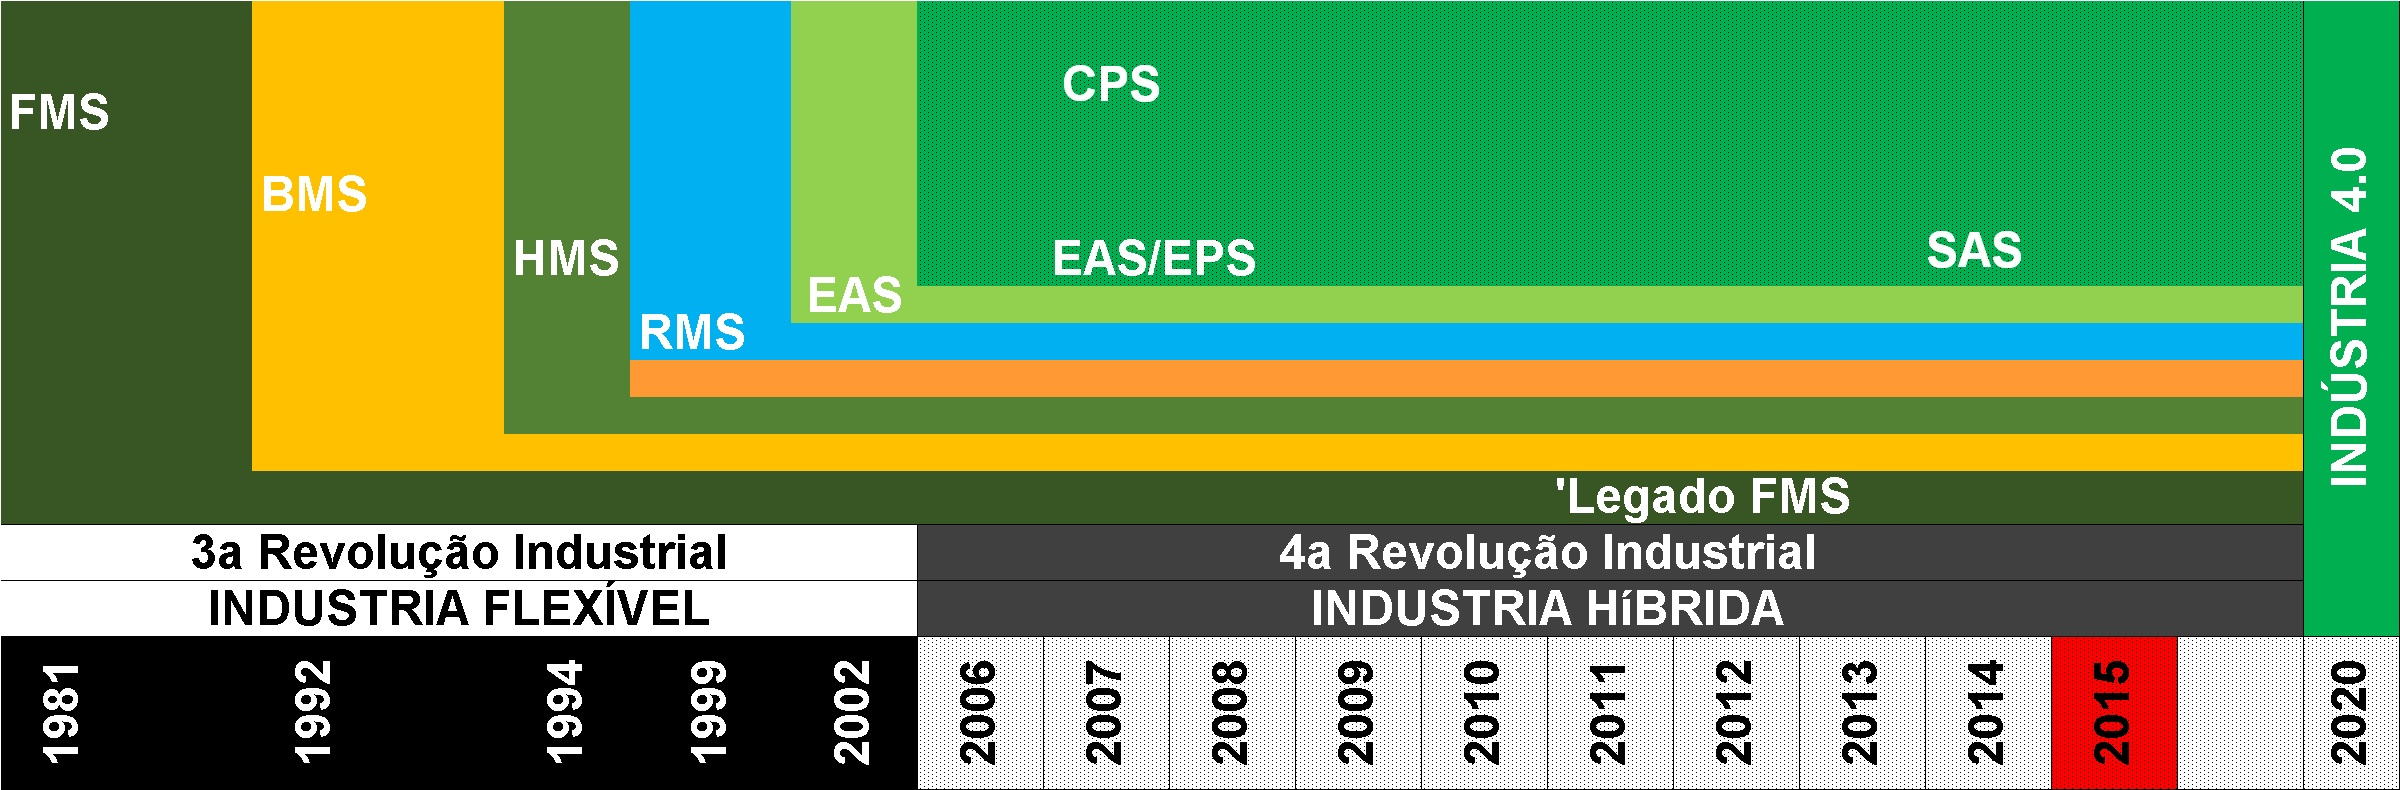
\includegraphics[width=\textwidth]{img/F0_MeDSE_PARADIGMAS_0_V2.jpg} 
	\caption{SIAPE: Paradigmas de produção}
	\label{fig:paradigmas_producao}
\end{figure*}
%================================================================
 
 
%===================================================================

\subsection{União Europeia (UE)}

%%==========================================================

\begin{figure*}[b]
	\centering
	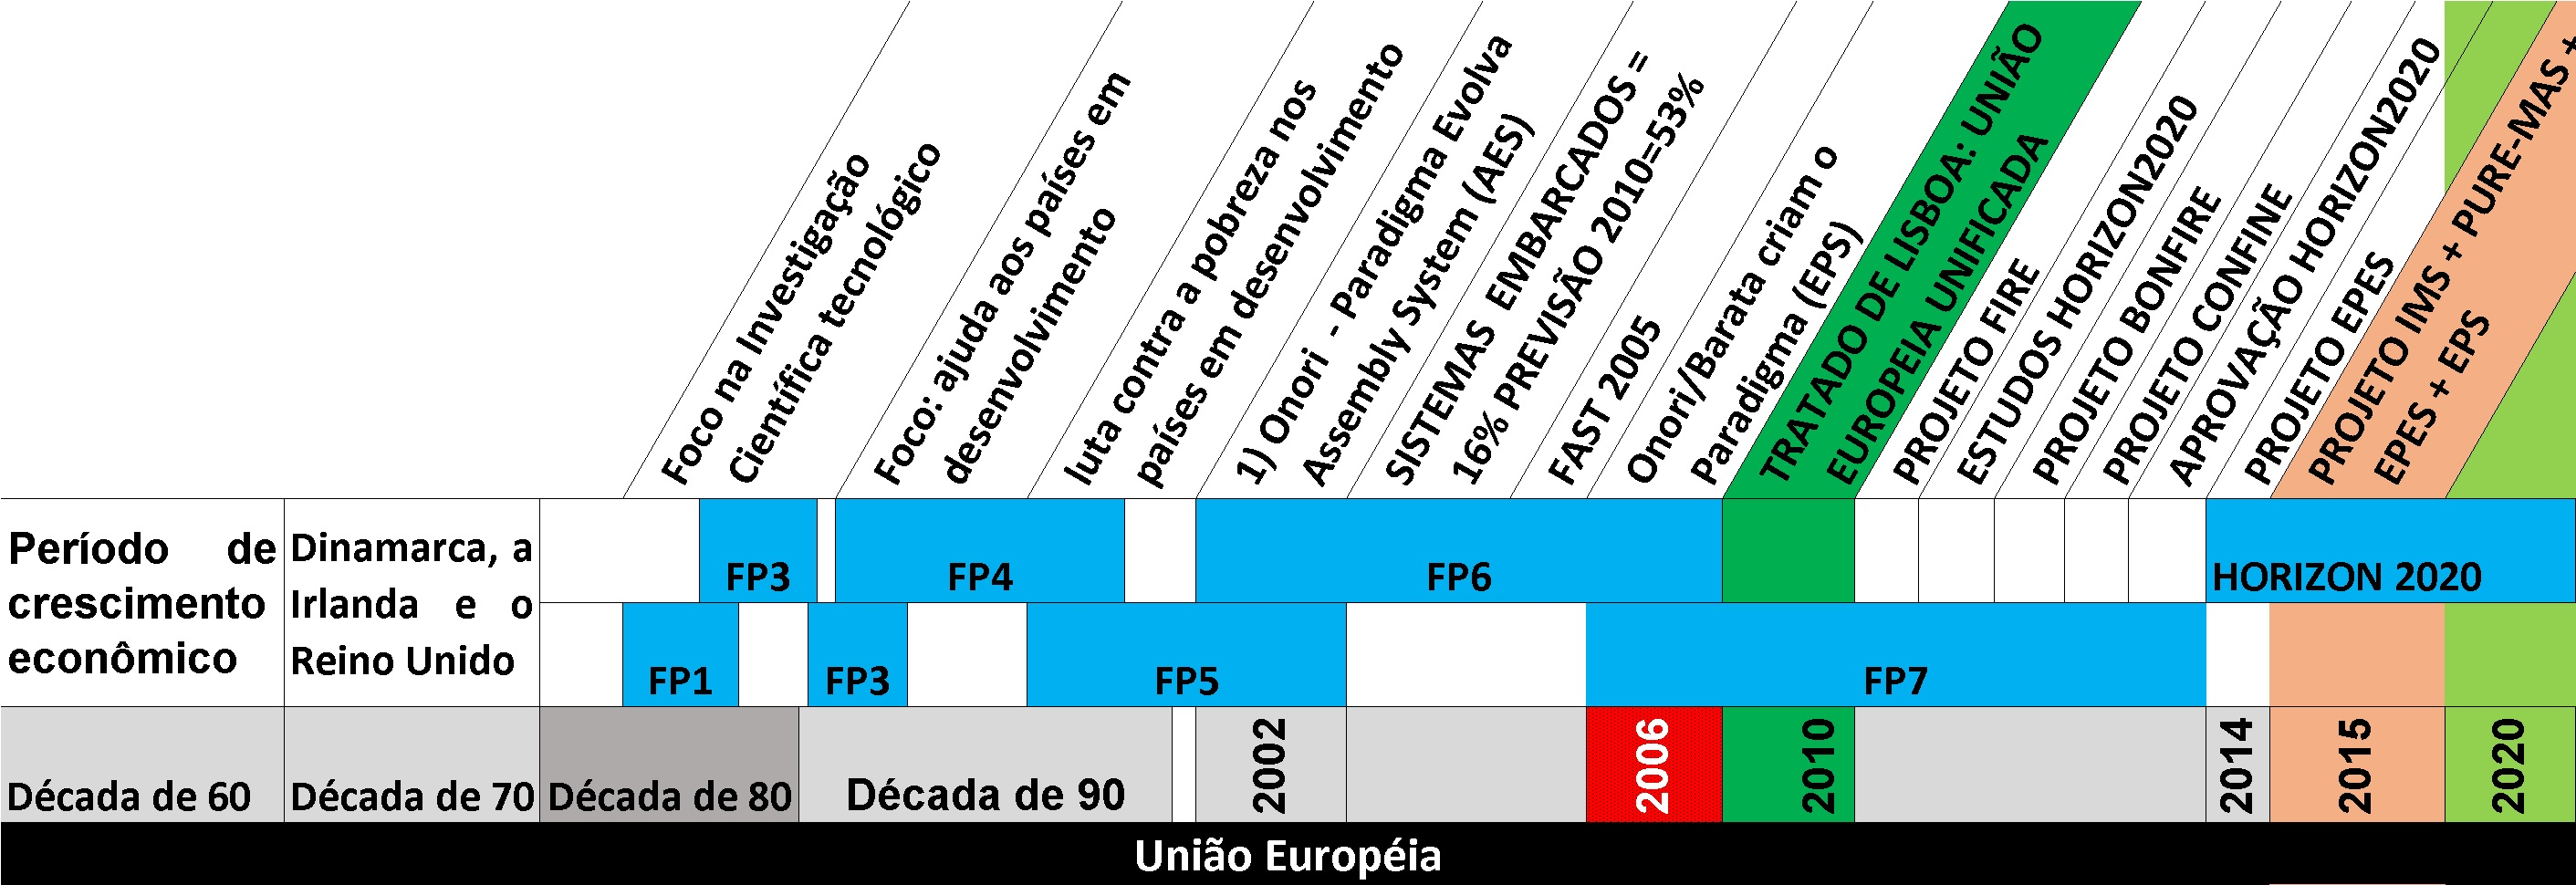
\includegraphics[width=\textwidth]{img/F1_MeDSE_UE.jpg} 
	\caption{Projetos Europeus e os sistemas evolutivos}
	\label{fig:projetos_europeus}
\end{figure*}

%%==========================================================

A Figura~\ref{fig:projetos_europeus} ilustra os principais eventos nos limites da UE e identifica os vários programas desenvolvidos desde a década de 80 até o ano 2020. Nela, igualmente, a criação do paradigma EPS em 2006 por Onori é enfatizada, assim como o Tratado de Lisboa em 2010 que concretizou a União Europeia como um bloco e possibilitou a posterior aprovação em 2013 do Programa Horizon 2020 -- com vigência de 2013 a 2020 -- que contempla os principais projetos que estão em desenvolvimento para formar os ambientes necessário para a Indústria 4.0.



%===================================================================

\subsection{Estados Unidos da América (EUA)}

A busca pela hegemonia científica e tecnológica nos EUA uniu as agências científicas, tecnológicas, militar, espacial e de segurança norte-americanas em torno das ciberestruturas~\cite{NITRDGROUPS2003}.

A Figura~\ref{F2} ilustra uma análise sobre o desenvolvimento das ciberestruturas desde a década de 60 até 2020, momento em que alguns projetos estarão sendo revisados ou concluídos. As principais iniciativas e projetos que motivaram o surgimento dos \textit{Cyber Physical System (CPS)}. O período inicia na década de 60 e se prolonga até o 2020, momento que alguns projetos estarão sendo revisado ou concluídos. Nota-se claramente que desde a década de 60 os EUA investem maciçamente nos centros de computação acadêmica, culminando na criação da ciência da computação, iniciativas em computação avançada e na criação da Internet.

Alguns marcos importantes igualmente anotados na Figura~\ref{F2}: em 2006 Hellen Gill da \textit{National Fundation Science (NFS)} cunha o termo \textit{Cyber Physical System (CPS)}~\cite{GILL2005}; em 2007 o nasce Conselho de Ciência em ciberinfraestrutura; em 2008 a comunidade acadêmica pressionou o governo~\cite{LEE2008} para uma reação conjunta; a partir de 2010 os orçamentos e projetos nos Estados unidos foram direcionados aos projetos \textit{CPS}.

\begin{figure*}[h]
	\centering
	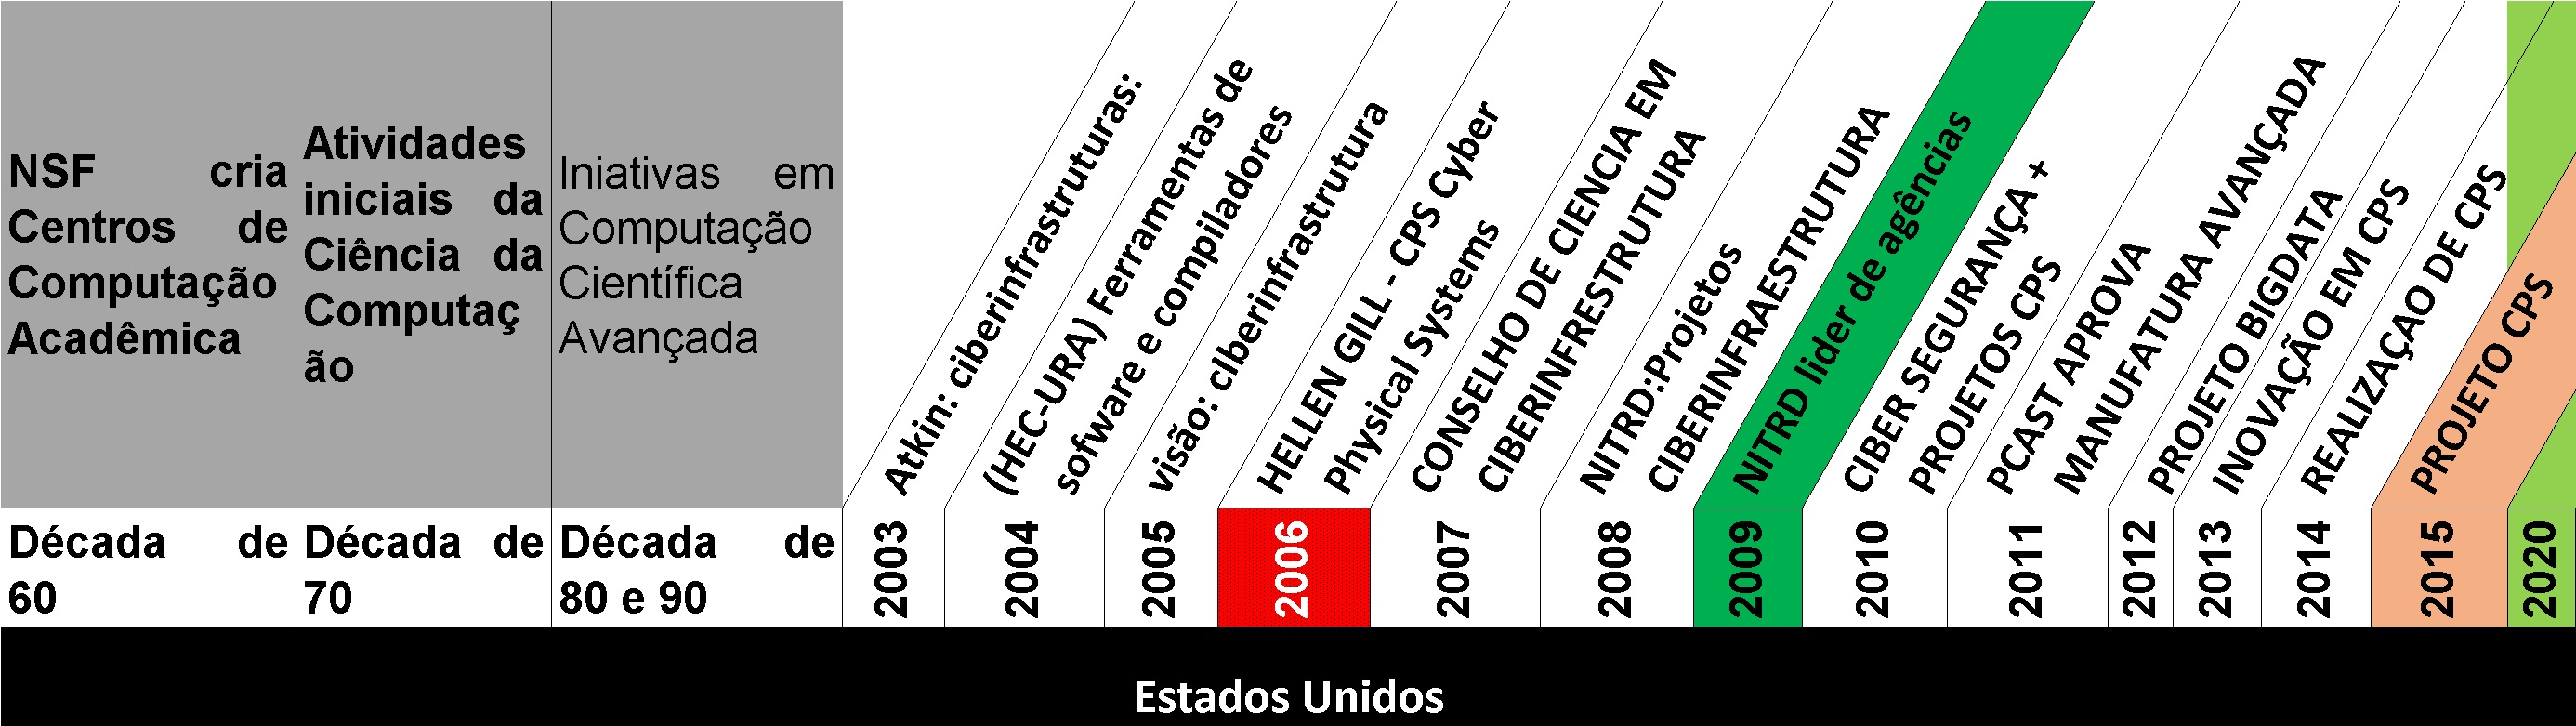
\includegraphics[width=\textwidth]{img/F2_MeDSE_USA1.jpg} 
	\caption{EUA: Linha do tempo dos CPS}
	\label{F2}
\end{figure*}


%===================================================================

\subsection{Brasil: Saindo da Indústria Mecânica e se estabelecendo na Indústria Flexível }	 


Analisando-se documentos oficiais do governo~\cite{PRESIDENCIADAREPUBLICA2014a}, os projetos, programas e estratégias em curso pelo Governo Brasileiro não evidenciam a inclusão do Brasil no círculo de países que iniciarão dentro da Plataforma da Indústria 4.0, isso dado o seu distanciamento tecnológico, a falta de sistemas baseados nos paradigmas emergentes, das fábricas inteligentes e a falta de integração entre as metas do Governo, da Indústria~\cite{CNI2013} e da Academia~\cite{CAPESVI2011}. Essa falta de integração e interação de estratégias, em moldes como acontecido na UE e EUA, condicionará o Brasil a receber o legado da Indústria Flexível e permanecer à margem da Indústria 4.0.


%===========================================================================================================

A Figura~\ref{fig:brasil_atraso} ilustra a contextualização da Indústria Brasileira que ainda está se adequando à Indústria Flexível. Nesta figura pode-se ver as chamadas revoluções industriais, que são identificadas por R1, R2, R3 e R4.  A fase entre R3 e R4 aqui é definida aqui como \emph{Indústria Híbrida}, dada a condição de sobrevivência, no mesmo espaço industrial de vários dos paradigmas de manufaturas até então conhecidos.

É importante notar que o Brasil ainda detém em grande parte de seu parque industrial sistemas legados da Indústria Mecânica e está se estabelecendo na Indústria Flexível, enquanto o mundo industrializado está totalmente incorporado aos sistemas flexíveis e experimentam a Indústria Híbrida, onde coexistem os sistemas flexíveis, ágeis, ciber e evolutivos. A marca R4 representa uma situação futura, a Indústria 4.0, onde sobreviverá a indústria inteligente, a saber àquela acoplada aos ciberespaços, contendo as ciberestruturas~\cite{Atkins2003}, os dispositivos e tecnologias que serão utilizados pelas fábricas inteligentes, que por sua vez, são baseados nos paradigmas evolutivos e nos \textit{Cyber-Physical Systems}~(CPS)~\cite{LEE2008}.

%===========================
\begin{figure*}
	\centering
	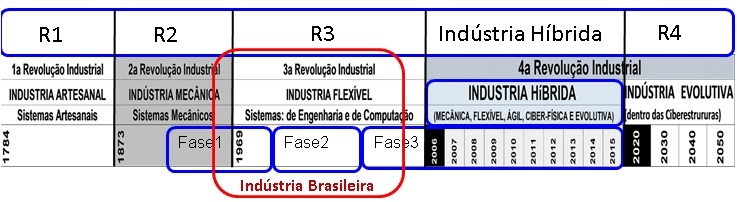
\includegraphics[width=16cm, height=5cm]{img/F3_MeDSE_GIB.jpg} 
	\caption{Brasil: Atraso da Indústria Brasileira}
	\label{fig:brasil_atraso}
\end{figure*}

%==========================================================================================================


%%========================================================================================================
\section{Tema e Problema}

Em ambientes industriais, a constante necessidade de reconfiguração das linhas de montagens é um problema recorrente. Nas atividades como a reprogramação das ferramentas de automação, braços robóticos e treinamentos de operadores de montagem, a reconfiguração é uma necessidade. Reduzir ou eliminar o tempo necessário para a reconfiguração requer mais que máquinas flexíveis, requer uma nova visão, um novo paradigma para as fábricas, bem como todo o ferramental para a aplicação deste paradigma.  		


\subsection{Delimitação do tema}
		
Considerando a contextualização global, delimitou-se o tema como \emph{Os sistemas evolutivos no contexto da Indústria 4.0 no Brasil.} 


\subsection{Especificação do problema}

Como foi colocado anteriormente, existe um problema no Brasil que é \emph{a inexistência de protótipos, no meio acadêmico e industrial, que reproduzam as propriedades dos sistemas evolutivos \textit{ (Evolvable Production System -- EPS)} a fim de permitir estudos e pequisas nas áreas de automação, controle e sistemas multi-agentes, protótipos estes capazes de ensejar a diminuição do gap tecnológico do Brasil.}

 	
\subsection{Questões de pesquisa (QP) e hipóteses relacionadas (HR)}	

	
\emph{QP1} -- Quais as características dos sistemas ágeis que podem evidenciar um sistema evolutivo de produção?
	
\emph{HR1} -- A adaptabilidade, conseguida através da reconfiguração dos parâmetros do sistema, evidenciará um sistema evolutivo de produção.

\emph{HR2} -- A evolutividade é realizada por meio da inclusão ou exclusão de módulos sem comprometer a eficiência e o funcionamento do sistema.


\subsection{Objetivo geral e específicos} 

Para realizar e comprovar essas hipóteses os seguintes objetivos foram definidos:

\begin{description}
	\item[Objetivo geral -] 
	\emph{Desenvolver um protótipo de sistema evolutivo  brasileiro baseado no paradigma \textit{EPS}}.
	
	\item[Objetivos específicos]:\par 
	
	\begin{enumerate}
	
		\item Desenvolver o módulo mecânico intercambiável, com interface elétrica;
		
		\item Desenvolver berço mecânico, com interface elétrica, para o módulo intercambiável;
		
		\item Desenvolver um protótipo que represente a indústria~3.0~\textit{(I3.0)};
		
		\item Desenvolver no PC a programação do agente de produto, consoante o paradigma EPS;
		
		\item Desenvolver no PC a programação do agente de recurso, consoante o paradigma EPS;
		
		\item Desenvolver programa de agentes que conversam entre si através do padrão FIPA;
		
		\item Desenvolver o acesso hardware programado via Raspberry Pi usando Java;
		
		\item Desenvolver interface SIAPE com o usuário para realizar o plug-and-produce; 
	 
	\end{enumerate}
	
\end{description} 


\section{Proposta do trabalho de dissertação}



\subsection{A proposta do projeto}
\label{subsec:a_proposta_projeto}

As recomendações da Indústria 4.0 \cite{VDE2014} apontam para propriedades dos Sistemas Evolutivos. Os Sistemas Evolutivos são baseados em agentes inteligentes e autônomos que, interagindo entre si, realizam a cooperação de agentes mecatrônicos para a execução de um objetivo bem definido. Os sistemas evolutivos tem duas capacidades fundamentais: a capacidade de \textit{adaptação} e a capacidade de \textit{evolução}.{\tiny }

%Por \textit{adaptação} entende-se que o sistema é capaz de propor uma configuração alternativa de si mesmo para minimizar os efeitos adversos de perturbações. Adaptação é de curto prazo e, normalmente, implica \textit{auto-reconfiguração} na forma de ajustes de parâmetros.
%
%Já o termo \textit{evolução} refere-se ao sistema que é capaz de permitir a introdução ou remoção de módulos existentes sem implicar na perda de performance e/ou quebra do seu funcionamento. A evolução se caracteriza num processo de longo prazo, podendo o sistema evoluir até o limite da tecnologia ou ao limite da planta fabril.
%
%Pode-se analisar tais capacidades através dos seguintes parâmetros: 
%
%\begin{itemize}
%	\item \textit{modularidade} que denota a noção de independência entre os módulos dos sistema; 
%	
%	\item \textit{granularidade} que evidencia o quanto de informação um agente deve possuir sobre os demais agentes, e a quantidade destes, a fim de se conseguir um objetivo definido; granularidade pode ser grossa quando, por exemplo, pouca informação e poucos agentes são necessários em uma coalizão, ou fina, quando, por exemplo, uma quantidade grande de agentes e muita informação sobre eles é necessária numa coalizão.
%	
%	\item \textit{plugabilidade} que é o conceito \textit{plug-and-produce} em tempo de produção e representa a capacidade de um módulo ser inserido ou retirado do sistema sem afetar a sua funcionalidade, ou mesmo a sua performance;
%\end{itemize}
%
%Quando se diz que um sistema é \textit{reconfigurável} isto significa que este possui a habilidade de redesenhar seu layout sem comprometer o funcionamento do sistema. Então, a plugabilidade é uma forma de reconfigurabilidade.
%	
%Quando um sistema possuir algum grau desses parâmetros, ele é dito ser \textit{auto-organizado}. Sistema auto-organizáveis são naturalmente \textit{dinâmicos}. Sistemas evolutivos possuem modularidade, plugabilidade, reconfigurabilidade e a sua granularidade pode ser ajustada conforme a complexidade do sistema.

Este trabalho visa, pois, o desenvolvimento de um sistema deste tipo, o \textbf{Sistema Inteligente Ágil de Processo Evolutivo (SIAPE)}~que é formado por uma planta composta de quatro partes que funcionam integradamente para reproduzir as duas características básicas dos sistemas EPS e pode ser analisado mediante estes quatro parâmetros.

O sistema é capaz de realizar a produção de anagramas que podem conter as seguintes letras: A, F, M, T, U. Essas letras são carimbadas em uma folha de papel contida em um carro que movimenta-se em uma esteira. Tais letras representam os processos que são realizados em sistemas industriais reais. Esses módulos são implementados como agentes inteligentes, e podem ser inseridos ou subtraídos do sistema para a concretização dos anagramas (produtos) e nas quantidades que se queira (lotes de produção), a partir de ordens de produção. Tais ordens são organizadas autonomamente em planos de produção de produtos. Quando há uma mudança na produção, isto é, a entrada de outra ordem para um novo anagrama, com quantidades diferentes, o sistema não tem a necessidade de reconfiguração entre tais produtos e lotes. E, finalmente, deve contar com o \textit{plug-and-produce}, isto é, na necessidade de uma letra desenvolvida posteriormente ao próprio sistema de montagem, este deve ser capaz de operar com a entrada de novos módulos de letras (em nosso exemplo: ``E'') como parte de seu funcionamento normal.


%==============================================================

\subsection{Metodologia da pesquisa}

A Figura \ref{fig:metodologia} ilustra a metodologia e facilita o entendimento entre os dois processos utilizados no desenvolvimento do SIAPE.

\begin{figure*}[h]
	\centering
	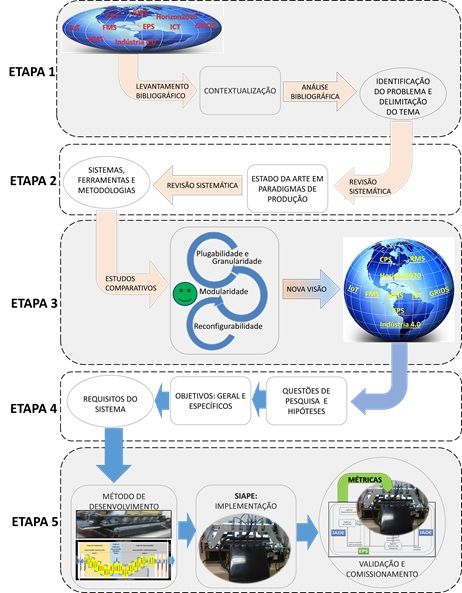
\includegraphics[height=0.8\textheight]{img/F4_SIAPE_METODOLOGIA_V0.jpg} 
	\caption{SIAPE - Metodologia da pesquisa}
	%\footnotesize{Fonte: Adaptado de~\cite{MUNZLINGER2012,MONTEBELO2000,SAMPAIO2007}}
	\label{fig:metodologia}
\end{figure*}

\begin{enumerate}
	
	\item ETAPA 1 - Objetivou o estudo do cenário atual como forma de evidenciar os principais pontos para a contextualização, e nos limites dessa, identificar um problema para ser tratado e a delimitação do tema da pesquisa.
	
	\item ETAPA 2 - Objetivou evidenciar o estado da arte considerando o tema delimitado, e baseado neste a elaboração das questões de pesquisa e hipóteses.
	
	\item ETAPA 3 - Nesta etapa foram definidas as propriedades e características que deveriam estar presentes no sistema desenvolvido.
		
	\item ETAPA 4 - Essa etapa teve como meta a elaboração dos requisitos, a partir das questões de pesquisas e das hipóteses relacionadas.
			
	\item ETAPA 5 - Nessa etapa o sistema foi implementado seguindo um método de desenvolvimento,  foram realizadas experimentações e o sistema foi validado por meio das métricas previamente definidas.
	
\end{enumerate}	
	
A Etapa 4 forneceu os requisitos do sistema com bases nas questões de pesquisa e nos objetivos geral e específicos. Esses requisitos foram tratados por um método de desenvolvimento também criado, por necessidade, para o desenvolvimento de sistemas evolutivos; o método realiza, de uma forma sistematizada, o desenvolvimento de um EPS por meio de três fases: a fase de concepção do sistema, a fase de implementação e a fase de comissionamento e finalização. Este método é explicado no Capítulo 3 e uma aplicação dele no desenvolvimento do SIAPE encontra-se detalhado no Capítulo 4.
	 

\subsection{Contribuições relevantes } 

Pode-se enumerar, dentre outras, as seguintes contribuições deste trabalho:

\begin{enumerate}
\item os dois protótipos: um flexível para reproduzir a condição atual da Indústria 3.0 (\iTresZero) e um evolutivo, que comporte as propriedades do paradigma EPS e da Plataforma da Indústria 4.0, que podem auxiliar projetistas, especialistas e acadêmicos no estudo de sistemas evolutivos;

\item uma arquitetura para os sistemas evolutivos que integre as recomendações da Indústria 4.0 (\iQuatroZero) com a performance do paradigma evolutivo de produção;

\item a metodologia para desenvolvimento de sistemas evolutivos.
\end{enumerate}
%========================================================================

\clearpage
\section{Organização do trabalho}

%\phl{Refazer, conforme o caso}

%\hl{OK. Aguardarei o término das revisões para processar este item}.

Este capítulo foi elaborado para descrever um breve resumo da contextualização global, identificar o tema e delimitar o problema a ser tratado, as questões de pesquisa utilizadas, os objetivos geral e específicos da proposta de trabalho,além das motivações e a metodologia utilizada. Os capítulos restantes desse trabalho estão dividido conforme segue. 

A Revisão da Literatura está descrita no Capítulo 2 que identifica as três revoluções industriais e alguns pontos que evidenciam a 4ª Revolução Industrial. Apresenta uma seção sobre EPS, objeto desta pesquisa. A conceituação teórica de alguns termos importantes e, finalmente, alguns trabalhos e pesquisas que se configuram como o estado da arte em sistemas evolutivos.

O Capítulo 3 descreve o desenvolvimento do SIAPE  e o método de desenvolvimento que foi criado para desenvolvê-lo.

No Capítulo 4 encontra-se a experimentação realizada por meio de um estudo de caso elaborado para evidenciar a operacionalidade do sistema.

No Capítulo 5 alguns resultados da experimentação são analisados, o sistema validado, e também são feitas alguns discussões em torno dos  resultados conseguidos na experimentação.

As conclusões encontram-se registradas no Capítulo 6, além dos trabalhos futuros que possam ser desenvolvidos a partir dos resultados desse trabalho de pesquisa.